\section{Results}
\label{sec:results}

\Tabref{tab:verdicts} summarizes our verdicts, and \figref{fig:quality} shows the main pattern: quality holds near each model's peak and then falls, at a point that differs by model and task. \Figref{fig:curves} shows all raw curves. Quality falls most abruptly on stories and more gradually on QA.

\begin{table}[t]
    \centering
    \small
    \resizebox{\textwidth}{!}{%
    \begin{tabular}{@{}>{\raggedright\arraybackslash}p{5.2cm}>{\raggedright\arraybackslash}p{2.5cm}>{\raggedright\arraybackslash}p{6.6cm}@{}}
        \toprule
        \textbf{Claim} & \textbf{Verdict} & \textbf{Evidence} \\
        \midrule
        H1: open-ended diversity plateaus above 1.2, coherence drops 20--40\% & Partly supported & Measured diversity stops rising in 9/10 models but peaks at $T$ = 1.0--1.4 and then falls. Judge coherence falls 48--62\% at $T = 1.4$ in 9/10 models. \\
        H2: above 0.7, QA accuracy degrades with no diversity gain & Mostly supported, small effect & Accuracy at $T$ = 0.8--1.0 is lower in all 10 models, significantly in 9, by at most 5.2 points. \coverfour stops improving above 0.7. \\
        H3: code has useful range 0.2--0.6, collapse above 0.8 & Refuted as stated & No significant drop from 0.6 to 0.8. \Tlo = 0 everywhere. Four models reach \Tu of 1.07--1.42. \\
        H4: smaller models have narrower useful ranges & Supported for Qwen, weak for Llama & Qwen: all three tasks. Llama: QA only. \\
        H5: curve shape differs across families & Supported & Llama gaps are 4--7 times the seed floor. Qwen and Mistral are close to each other. \\
        \bottomrule
    \end{tabular}
    }
    \caption{Verdict on each clause of the hypothesis.}
    \label{tab:verdicts}
\end{table}


\begin{figure}[t]
    \centering
    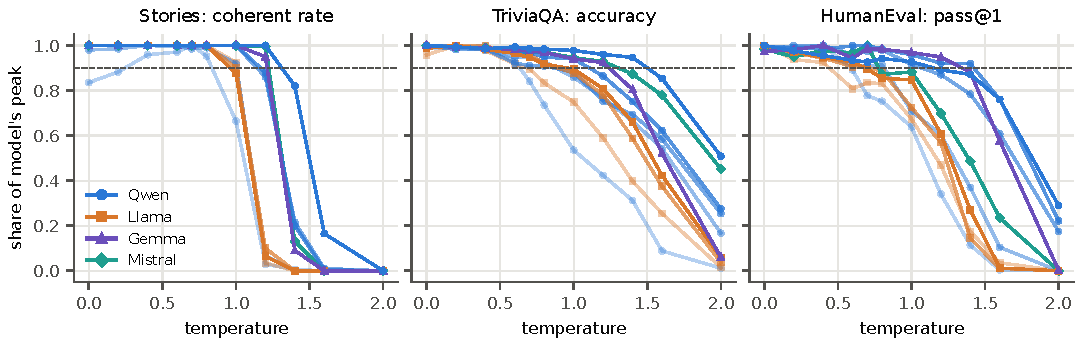
\includegraphics[width=0.95\linewidth]{figures/quality_normalized.pdf}
    \caption{Quality relative to each model's own peak, with darker lines for larger models in a family. The dashed line marks 90\%, which defines \Tu. On stories, most models go from near their peak to near zero within one or two grid steps, and the break ranges from $T \approx 0.8$ to 1.3 across models.}
    \label{fig:quality}
\end{figure}

\begin{figure}[t]
    \centering
    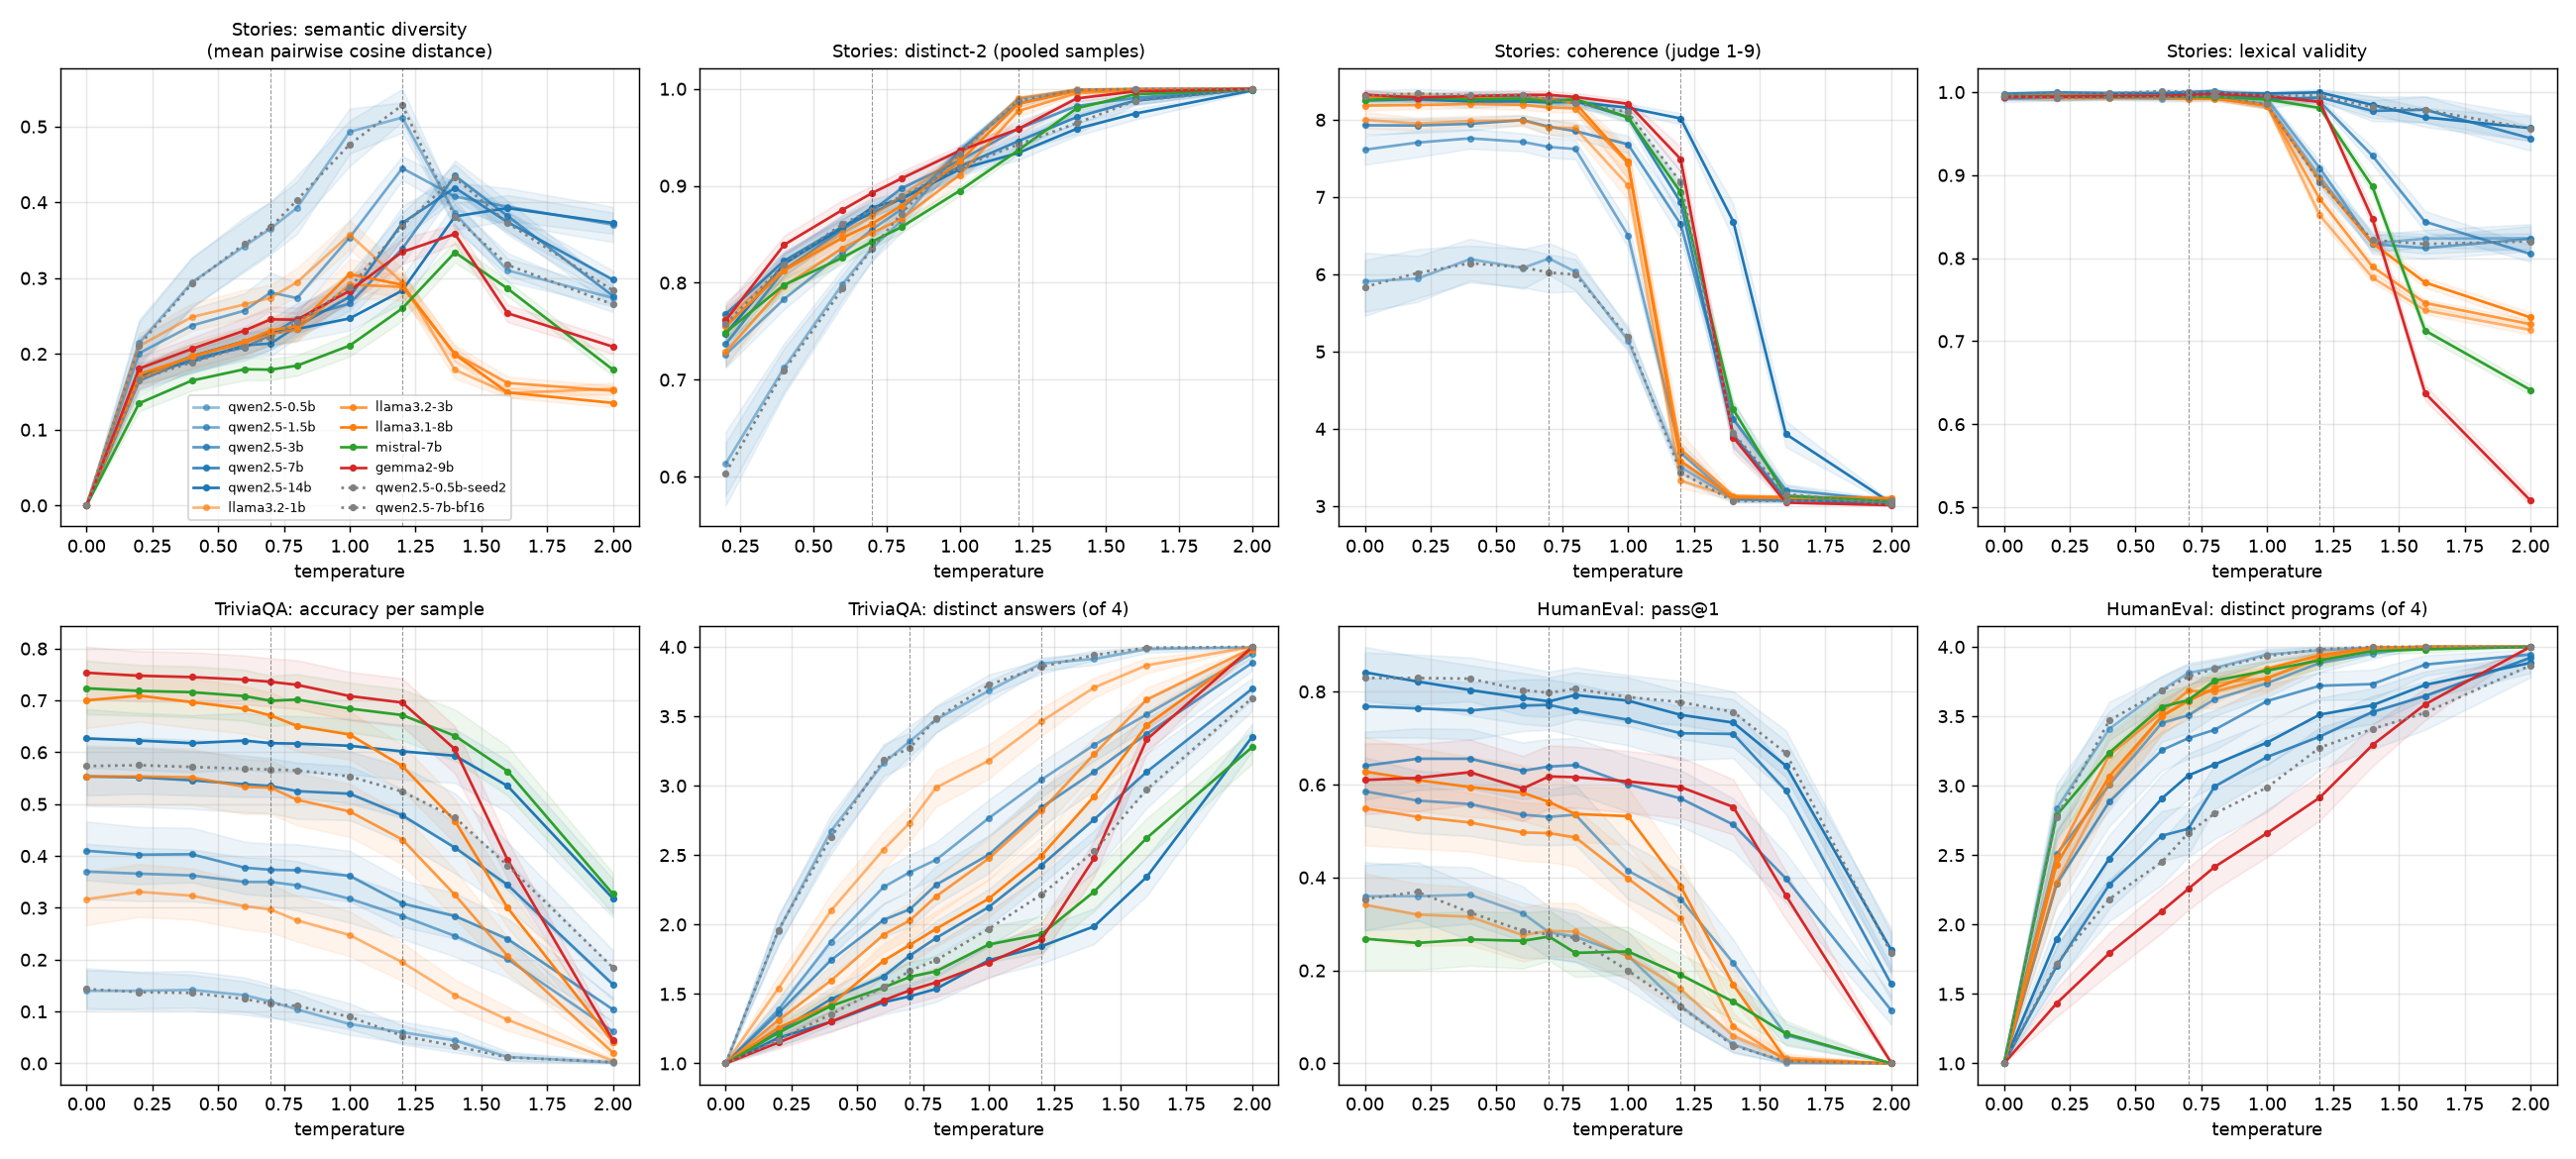
\includegraphics[width=0.95\linewidth]{figures/curves_all.png}
    \caption{All metrics by temperature for all models and controls, with bands showing bootstrap 95\% CIs. Vertical dashed lines mark $T = 0.7$ and $1.2$. Dotted gray lines are the control runs, which closely follow the matching main runs in shape.}
    \label{fig:curves}
\end{figure}

\subsection{H1: open-ended generation}
\label{sec:h1}

{\bf Does diversity plateau above 1.2?} In a sense it does, but ``plateau'' is the wrong shape. Semantic diversity rises, peaks at $T$ of 1.0--1.4, and then falls in 9 of 10 models (\tabref{tab:stories}). Qwen2.5-14B is the exception, with no slowdown between the two ranges (ratio 0.98, 95\% CI 0.69--1.30).

\begin{table}[t]
    \centering
    \resizebox{\textwidth}{!}{%
    \begin{tabular}{@{}lccccccccc@{}}
        \toprule
        & & \multicolumn{2}{c}{\textbf{Slope ratio}} & \multicolumn{3}{c}{\textbf{Judge drop from peak}} & \multicolumn{2}{c}{\textbf{Coherent rate}} \\
        \cmidrule(lr){3-4} \cmidrule(lr){5-7} \cmidrule(lr){8-9}
        \textbf{Model} & \textbf{Peak diversity $T$} & Semantic & Distinct-2 & $T$=1.2 & $T$=1.4 & $T$=2.0 & $T$=1.2 & $T$=1.4 \\
        \midrule
        Qwen2.5-0.5B & 1.2 & $-$1.00 & 0.03 & 44\% & 50\% & 50\% & 0.03 & 0.01 \\
        Qwen2.5-1.5B & 1.2 & $-$0.38 & 0.07 & 53\% & 60\% & 61\% & 0.07 & 0.00 \\
        Qwen2.5-3B & 1.4 & $-$0.45 & 0.23 & 17\% & 48\% & 62\% & 0.86 & 0.22 \\
        Qwen2.5-7B & 1.4 & $-$0.47 & 0.38 & 17\% & 53\% & 64\% & 0.88 & 0.20 \\
        Qwen2.5-14B & {\bf 1.6} & {\bf 0.98} & {\bf 0.43} & {\bf 3\%} & {\bf 19\%} & 63\% & {\bf 1.00} & {\bf 0.82} \\
        Llama-3.2-1B & 1.0 & $-$2.09 & 0.05 & 58\% & 61\% & 62\% & 0.04 & 0.00 \\
        Llama-3.2-3B & 1.0 & $-$1.41 & 0.12 & 55\% & 62\% & 62\% & 0.10 & 0.00 \\
        Llama-3.1-8B & 1.0 & $-$1.65 & 0.09 & 57\% & 62\% & 63\% & 0.07 & 0.00 \\
        Mistral-7B & 1.4 & $-$0.81 & 0.42 & 15\% & 49\% & 63\% & 0.995 & 0.13 \\
        Gemma-2-9B & 1.4 & $-$1.02 & 0.26 & 10\% & 53\% & 64\% & 0.95 & 0.09 \\
        \bottomrule
    \end{tabular}
    }
    \caption{Open-ended generation. The slope ratio divides the diversity slope over $T \in [1.2, 2.0]$ by the slope over $[0.2, 1.2]$. Most models lose about half their judge score by $T = 1.4$, and the coherent rate shows the loss is near total. Best value in each column is in \textbf{bold}, except at $T = 2.0$, where all models sit at the judge's floor.}
    \label{tab:stories}
\end{table}


Most of this pattern comes from the measures, not the models. Distinct-2 flattens because it reaches its ceiling of 1.0. We read the fall in semantic diversity as an embedding artifact: degenerate text appears to embed similarly whatever it says, so a falling score does not mean outputs are less varied. We did not test this reading directly. Restricting to prompts where both judged samples are coherent supports it, because semantic diversity then rises at almost every temperature until too few coherent groups remain. For example, Gemma rises from 0.18 at $T = 0.2$ to 0.37 at $T = 1.4$. This is a selected subset, but it suggests that coherence loss, not saturation, ends useful diversity (\figref{fig:frontier}).

\begin{figure}[t]
    \centering
    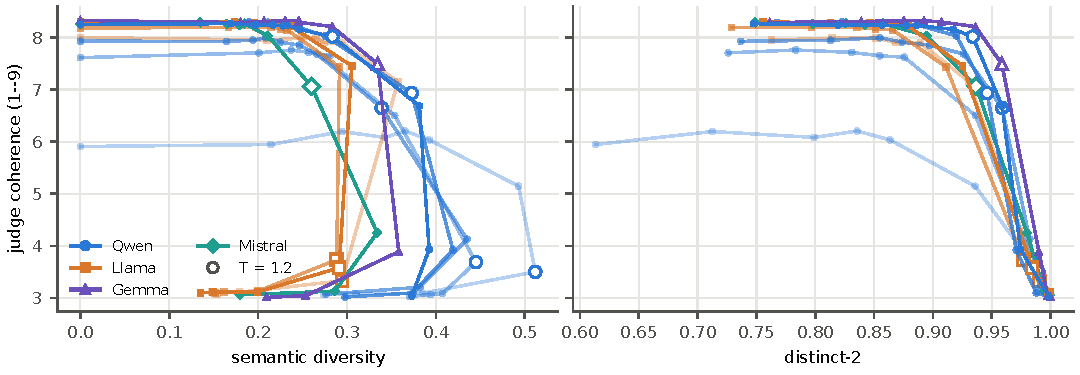
\includegraphics[width=0.95\linewidth]{figures/story_frontier.pdf}
    \caption{Diversity against coherence as $T$ rises, with hollow markers at $T = 1.2$. Coherence stays flat while diversity rises, then drops steeply. \figleft: semantic diversity turns back on itself past the cliff. \figright: distinct-2 presses against its ceiling.}
    \label{fig:frontier}
\end{figure}

{\bf Does coherence drop 20--40\%?} This prediction is met only in passing. At $T = 1.4$ Qwen2.5-14B falls 19\%, close to the range, while the other nine models lose 48--62\%. These figures understate the damage: the judge rarely scores below 3, so the raw scale cannot fall more than about 64\%. The coherent rate shows it better, falling from about 1.0 to about 0 within one or two grid steps. For example, Mistral goes from 0.995 at $T = 1.2$ to 0.13 at $T = 1.4$.

\subsection{H2: factual QA}
\label{sec:h2}

{\bf Does accuracy degrade above 0.7?} Yes, but the loss is small (\tabref{tab:qa}). Accuracy at $T$ of 0.8--1.0 is below that at $T \le 0.7$ in all 10 models and significantly so in 9, by 2.0--5.2 points. Qwen2.5-14B loses 0.7 points, which is not significant ($p = .217$). The decline stays gradual up to about $T = 1.2$ and steepens beyond it.

{\bf Does the extra diversity help?} Below 0.7 it does: \coverfour at $T = 0.7$ is 2.7--9.7 points above greedy accuracy. Above 0.7 it does not. Moving from 0.7 to 1.0 changes coverage by $-$5.0 to +1.7 points, $-$0.8 on average, even though distinct answers keep rising. The extra diversity is mostly more wrong answers.

\begin{table}[t]
    \centering
    \resizebox{\textwidth}{!}{%
    \begin{tabular}{@{}lcccccccc@{}}
        \toprule
        & \multicolumn{3}{c}{\textbf{Mean accuracy}} & & & & \multicolumn{2}{c}{\textbf{\coverfour}} \\
        \cmidrule(lr){2-4} \cmidrule(lr){8-9}
        \textbf{Model} & Greedy & $T \le 0.7$ & $T$ 0.8--1.0 & \textbf{Diff.\ (pt)} & \textbf{Holm $p$} & $T \ge 1.2$ & $T$=0.7 & $T$=1.0 \\
        \midrule
        Qwen2.5-0.5B & .140 & .134 & .090 & $-$4.4 & $<$.001 & .030 & .217 & .167 \\
        Qwen2.5-1.5B & .370 & .360 & .330 & $-$2.9 & .001 & .198 & .467 & .430 \\
        Qwen2.5-3B & .410 & .393 & .367 & $-$2.6 & .001 & .234 & .447 & .463 \\
        Qwen2.5-7B & .553 & .545 & .522 & $-$2.2 & .001 & .348 & .593 & .603 \\
        Qwen2.5-14B & .627 & .621 & .615 & {\bf $-$0.7} & .217 & .512 & .653 & .660 \\
        Llama-3.2-1B & .317 & .314 & .262 & $-$5.2 & $<$.001 & .104 & .410 & .383 \\
        Llama-3.2-3B & .553 & .545 & .497 & $-$4.8 & $<$.001 & .246 & .613 & .623 \\
        Llama-3.1-8B & .700 & .692 & .642 & $-$5.0 & $<$.001 & .346 & .763 & .760 \\
        Mistral-7B & .723 & .713 & .693 & $-$2.0 & $<$.001 & {\bf .548} & .753 & .757 \\
        Gemma-2-9B & {\bf .753} & {\bf .744} & {\bf .719} & $-$2.5 & .001 & .435 & {\bf .810} & {\bf .800} \\
        \bottomrule
    \end{tabular}
    }
    \caption{Factual QA. The difference compares $T$ of 0.8--1.0 with $T \le 0.7$. Accuracy falls in every model and significantly in nine, but only by a few points. \coverfour shows no consistent gain from 0.7 to 1.0. $p$-values use 10,000 permutations, so ``$<$.001'' is near the resolution limit. Best values are in \textbf{bold}.}
    \label{tab:qa}
\end{table}


\subsection{H3: code generation}
\label{sec:h3}

{\bf Is there a sharp collapse just above 0.8?} No (\tabref{tab:code}). No model drops significantly from 0.6 to 0.8 after Holm correction. From 0.6 to 1.0 four models drop significantly, all at 3B or below, and the largest relative drop is 28\% (Qwen2.5-0.5B), under the 30\% we set as our example of a sharp drop in the plan.

{\bf Is the useful range 0.2--0.6?} The lower bound is not supported: $\Tlo = 0$ for every model, and five models reach their best \passone at greedy. The upper bound varies from 0.44 to 1.42, and Qwen2.5-3B, -7B, -14B and Gemma all stay within 90\% of peak to at least 1.07.

{\bf Where does temperature pay off?} It pays off when several attempts can be tested. At $T = 0.8$, \passfour exceeds greedy \passone by 6--18 points in every model, led by Qwen2.5-3B at +18.3. Across models, the best temperature for \passfour ranges from 0.4 to 1.4, and for five models it is 0.7 or 0.8.

{\bf Where is the real collapse?} It comes later and is syntactic (\tabref{tab:failures}). Pooled across models, syntax errors go from 2\% at $T = 0.8$ to 17\% at 1.2, 45\% at 1.4, and 93\% at 2.0.

\begin{table}[t]
    \centering
    \resizebox{\textwidth}{!}{%
    \begin{tabular}{@{}lccccccccccc@{}}
        \toprule
        & & & & & \multicolumn{4}{c}{\textbf{\passone}} & & \\
        \cmidrule(lr){6-9}
        \textbf{Model} & \textbf{Greedy} & \textbf{Best $T$} & \textbf{\Tu (95\% CI)} & \textbf{\Tfifty} & 0.6 & 0.8 & 1.0 & 1.2 & \textbf{\passfour at 0.8} & \textbf{Holm $p$, 0.6 vs.\ 1.0} \\
        \midrule
        Qwen2.5-0.5B & .360 & 0.4 & 0.58 (0.41--0.64) & 1.09 & .323 & .273 & .232 & .123 & .476 & $<$.001 \\
        Qwen2.5-1.5B & .585 & 0 & 0.81 (0.34--0.87) & 1.29 & .535 & .535 & .415 & .354 & .750 & $<$.001 \\
        Qwen2.5-3B & .640 & 0.2 & 1.07 (0.81--1.22) & 1.70 & .630 & .642 & .601 & .570 & .823 & .916 \\
        Qwen2.5-7B & .768 & 0.7 & {\bf 1.42} (1.07--1.46) & 1.79 & .770 & .759 & .739 & .710 & .860 & .392 \\
        Qwen2.5-14B & {\bf .841} & 0 & 1.15 (0.56--1.43) & {\bf 1.82} & {\bf .787} & {\bf .793} & {\bf .780} & {\bf .750} & {\bf .902} & .946 \\
        Llama-3.2-1B & .341 & 0 & 0.44 (0.16--0.68) & 1.17 & .276 & .284 & .230 & .160 & .421 & .038 \\
        Llama-3.2-3B & .549 & 0 & 0.72 (0.31--0.88) & 1.23 & .497 & .486 & .398 & .312 & .707 & $<$.001 \\
        Llama-3.1-8B & .628 & 0 & 0.69 (0.37--0.91) & 1.26 & .582 & .537 & .532 & .381 & .744 & .085 \\
        Mistral-7B & .268 & 0.7 & 0.78 (0.14--1.05) & 1.39 & .264 & .238 & .241 & .191 & .421 & .946 \\
        Gemma-2-9B & .610 & 0.4 & 1.34 (0.60--1.41) & 1.65 & .591 & .616 & .607 & .595 & .707 & .946 \\
        \bottomrule
    \end{tabular}
    }
    \caption{Code generation. Best $T$ maximizes \passone. Larger models hold their \passone far past $T = 0.8$, while the four significant drops from 0.6 to 1.0 are all at 3B or below. \Tu CIs are wide because curves are flat near the threshold. Best values are in \textbf{bold}.}
    \label{tab:code}
\end{table}


\subsection{H4: model size}
\label{sec:h4}

Larger models tolerate higher temperature in the Qwen family on all three tasks, though the code contrast only just clears zero and is not monotonic, since Qwen2.5-14B has a lower \Tu than Qwen2.5-7B (\tabref{tab:size}, \figref{fig:ranges}). In the Llama family the trend holds on QA only. Story \Tu is 1.01 at 1B, 1.00 at 3B, and 0.96 at 8B. Code \Tfifty, which is less sensitive than \Tu, also rises with size: 1.09 to 1.82 for Qwen and 1.17 to 1.26 for Llama. Spearman values within a ladder rest on 3--5 points, so we rely on the bootstrap contrasts instead.

\begin{table}[t]
    \centering
    \begin{tabular}{@{}lccc@{}}
        \toprule
        \textbf{Task} & \textbf{Qwen 0.5B$\to$14B $\Delta$\Tu} & \textbf{Llama 1B$\to$8B $\Delta$\Tu} & \textbf{Spearman $\rho$, 10 models ($p$)} \\
        \midrule
        Stories & +0.47 (0.43, 0.55) & $-$0.05 ($-$0.09, 0.00) & 0.61 (.060) \\
        QA & +0.87 (0.76, 1.11) & +0.27 (0.04, 0.48) & 0.90 ($<$.001) \\
        Code & +0.57 (0.00, 0.93) & +0.25 ($-$0.15, 0.59) & 0.64 (.048) \\
        \bottomrule
    \end{tabular}
    \caption{Size effects on \Tu, with 95\% CIs for the ladder contrasts. The Qwen ladder gains range on every task, though the code CI barely clears zero. The Llama ladder gains on QA only.}
    \label{tab:size}
\end{table}


\begin{figure}[t]
    \centering
    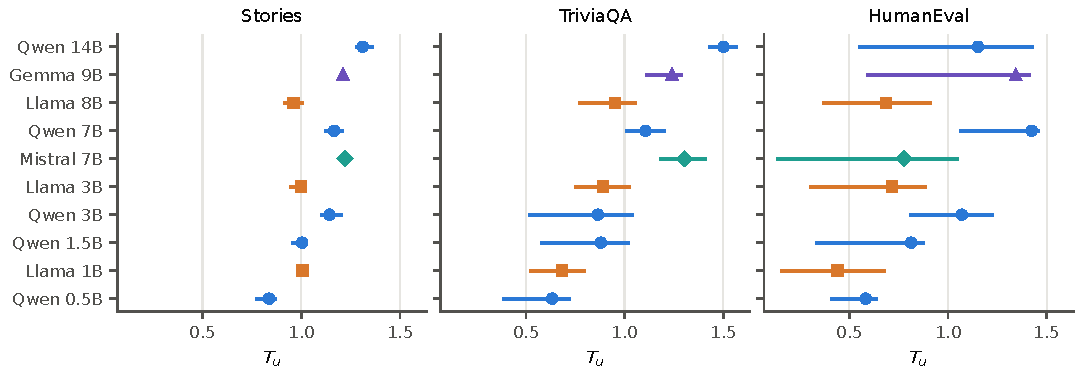
\includegraphics[width=0.95\linewidth]{figures/useful_ranges.pdf}
    \caption{Upper bound of the useful range for each model, ordered by size, with 95\% CIs. Story \Tu shows Llama holding near 1.0 at every size while Qwen climbs with size. Code CIs are wide, so single-model code comparisons are weak.}
    \label{fig:ranges}
\end{figure}

\subsection{H5: family differences at matched scale}
\label{sec:h5}

Curve shapes differ across families, but not evenly (\tabref{tab:family}, \figref{fig:family}). Llama differs from the other three families by 4--7 times the seed floor, and it peaks at $T = 1.0$ rather than 1.4. The 1--1.5B and 3B Qwen-versus-Llama pairs show the same result, with gaps of 0.225 and 0.224. Gemma sits between the groups, and Qwen and Mistral are close to each other.

\begin{table}[t]
    \centering
    \begin{tabular}{@{}lccc@{}}
        \toprule
        \textbf{Pair (7--9B, all AWQ)} & \textbf{Shape gap} & \textbf{$T$s with CI excluding 0} & \textbf{Peak $T$} \\
        \midrule
        Qwen 7B vs.\ Llama 8B & {\bf 0.220} & 9 & 1.4 vs.\ 1.0 \\
        Llama 8B vs.\ Mistral 7B & 0.205 & {\bf 10} & 1.0 vs.\ 1.4 \\
        Llama 8B vs.\ Gemma 9B & 0.118 & 8 & 1.0 vs.\ 1.4 \\
        Qwen 7B vs.\ Gemma 9B & 0.104 & 8 & 1.4 vs.\ 1.4 \\
        Mistral 7B vs.\ Gemma 9B & 0.098 & 9 & 1.4 vs.\ 1.4 \\
        Qwen 7B vs.\ Mistral 7B & 0.046 & 2 & 1.4 vs.\ 1.4 \\
        \midrule
        Floor: seed replicate & 0.031 & 0 & 1.2 vs.\ 1.2 \\
        Floor: bf16 vs.\ AWQ & 0.026 & 1 & 1.4 vs.\ 1.4 \\
        \bottomrule
    \end{tabular}
    \caption{Family differences in semantic diversity curves, out of the 10 temperatures above 0. Llama pairs with Qwen and Mistral sit far above both floors, and Qwen and Mistral sit close to them. The largest values are in \textbf{bold}.}
    \label{tab:family}
\end{table}


On stories, family matters more than size in this sample. Llama-8B breaks at $\Tu = 0.96$, close to Llama-1B at 1.01, while the other 7--9B models hold to 1.17--1.22. The evidence is weaker on the other two tasks: the seed floors for QA accuracy (0.061) and \passone (0.051) are larger, and the largest 7--9B gaps reach only 0.115 and 0.213.

\begin{figure}[t]
    \centering
    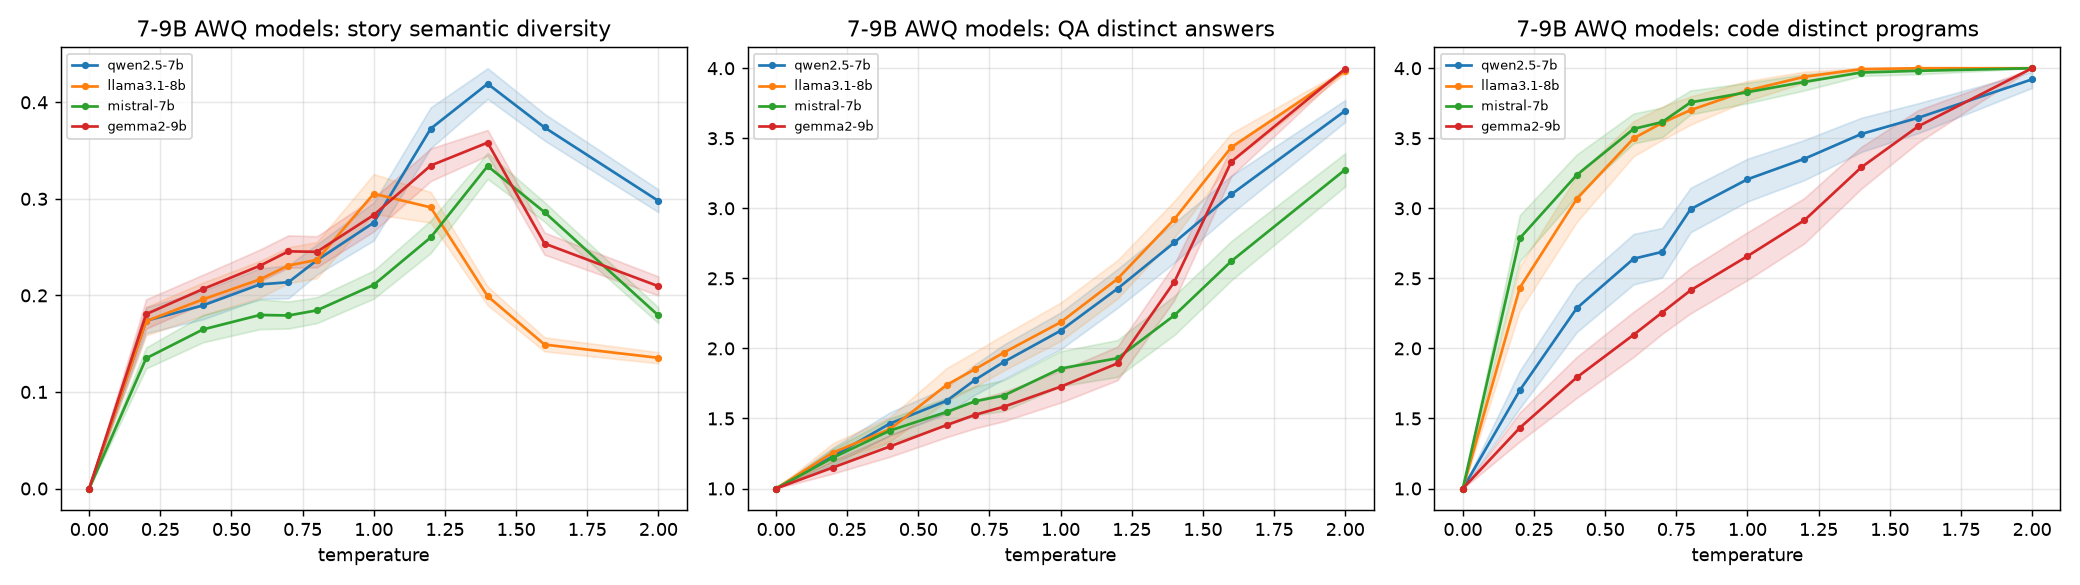
\includegraphics[width=0.95\linewidth]{figures/family_matched_diversity.png}
    \caption{Diversity curves for the four 7--9B AWQ models. On stories, Llama peaks and falls earlier than the others. On code, Llama and Mistral become diverse at low temperature, while Qwen and Gemma rise slowly, so the family order is not the same on each task.}
    \label{fig:family}
\end{figure}

\subsection{Controls and failure modes}
\label{sec:controls}

\para{Seed.} Two sampling-seed runs of Qwen2.5-0.5B differ at no temperature on any metric.

\para{Precision.} Comparing Qwen2.5-7B in bf16 and AWQ, curve shapes sit at the seed floor (semantic diversity gap 0.026). Levels do differ: greedy \passone is .829 versus .768, and greedy QA accuracy is .573 versus .553. AWQ therefore does not explain the shape differences above, but absolute levels should not be compared across precisions.

\para{Failure modes.} Above the cliff, models stop ending their outputs, drift into other languages, and emit code tokens in prose (\tabref{tab:failures}). Story truncation at the token limit goes from 14\% at $T = 1.0$ to 70\% at $T = 1.4$.

\begin{table}[t]
    \centering
    \begin{tabular}{@{}ccccccccc@{}}
        \toprule
        & \multicolumn{3}{c}{\textbf{Code}} & \multicolumn{2}{c}{\textbf{QA}} & \multicolumn{2}{c}{\textbf{Stories}} \\
        \cmidrule(lr){2-4} \cmidrule(lr){5-6} \cmidrule(lr){7-8}
        \textbf{$T$} & Passes & Syntax errors & Truncated & Correct & Rambling & Truncated & Non-ASCII \\
        \midrule
        0.7 & 52\% & 2\% & 2\% & 49\% & 3\% & 10\% & 0.1\% \\
        1.0 & 48\% & 4\% & 2\% & 47\% & 2\% & 14\% & 0.5\% \\
        1.2 & 42\% & 17\% & 9\% & 43\% & 4\% & 47\% & 1.7\% \\
        1.4 & 32\% & 45\% & 35\% & 37\% & 12\% & 70\% & 5.5\% \\
        1.6 & 21\% & 68\% & 61\% & 29\% & 28\% & 87\% & 9.0\% \\
        2.0 & 5\% & 93\% & 89\% & 11\% & 58\% & 92\% & 11.4\% \\
        \bottomrule
    \end{tabular}
    \caption{Failure modes pooled over the 10 main models. Rambling means a wrong QA answer of more than 8 words. Between $T = 1.0$ and $1.4$, models stop ending their outputs and code stops parsing.}
    \label{tab:failures}
\end{table}

